% Options for packages loaded elsewhere
\PassOptionsToPackage{unicode}{hyperref}
\PassOptionsToPackage{hyphens}{url}
%
\documentclass[
]{book}
\usepackage{amsmath,amssymb}
\usepackage{lmodern}
\usepackage{iftex}
\ifPDFTeX
  \usepackage[T1]{fontenc}
  \usepackage[utf8]{inputenc}
  \usepackage{textcomp} % provide euro and other symbols
\else % if luatex or xetex
  \usepackage{unicode-math}
  \defaultfontfeatures{Scale=MatchLowercase}
  \defaultfontfeatures[\rmfamily]{Ligatures=TeX,Scale=1}
  \setmainfont[]{Libre Baskerville}
\fi
% Use upquote if available, for straight quotes in verbatim environments
\IfFileExists{upquote.sty}{\usepackage{upquote}}{}
\IfFileExists{microtype.sty}{% use microtype if available
  \usepackage[]{microtype}
  \UseMicrotypeSet[protrusion]{basicmath} % disable protrusion for tt fonts
}{}
\makeatletter
\@ifundefined{KOMAClassName}{% if non-KOMA class
  \IfFileExists{parskip.sty}{%
    \usepackage{parskip}
  }{% else
    \setlength{\parindent}{0pt}
    \setlength{\parskip}{6pt plus 2pt minus 1pt}}
}{% if KOMA class
  \KOMAoptions{parskip=half}}
\makeatother
\usepackage{xcolor}
\usepackage{listings}
\newcommand{\passthrough}[1]{#1}
\lstset{defaultdialect=[5.3]Lua}
\lstset{defaultdialect=[x86masm]Assembler}
\usepackage{longtable,booktabs,array}
\usepackage{calc} % for calculating minipage widths
% Correct order of tables after \paragraph or \subparagraph
\usepackage{etoolbox}
\makeatletter
\patchcmd\longtable{\par}{\if@noskipsec\mbox{}\fi\par}{}{}
\makeatother
% Allow footnotes in longtable head/foot
\IfFileExists{footnotehyper.sty}{\usepackage{footnotehyper}}{\usepackage{footnote}}
\makesavenoteenv{longtable}
\usepackage{graphicx}
\makeatletter
\def\maxwidth{\ifdim\Gin@nat@width>\linewidth\linewidth\else\Gin@nat@width\fi}
\def\maxheight{\ifdim\Gin@nat@height>\textheight\textheight\else\Gin@nat@height\fi}
\makeatother
% Scale images if necessary, so that they will not overflow the page
% margins by default, and it is still possible to overwrite the defaults
% using explicit options in \includegraphics[width, height, ...]{}
\setkeys{Gin}{width=\maxwidth,height=\maxheight,keepaspectratio}
% Set default figure placement to htbp
\makeatletter
\def\fps@figure{htbp}
\makeatother
\setlength{\emergencystretch}{3em} % prevent overfull lines
\providecommand{\tightlist}{%
  \setlength{\itemsep}{0pt}\setlength{\parskip}{0pt}}
\setcounter{secnumdepth}{5}
\newlength{\cslhangindent}
\setlength{\cslhangindent}{1.5em}
\newlength{\csllabelwidth}
\setlength{\csllabelwidth}{3em}
\newlength{\cslentryspacingunit} % times entry-spacing
\setlength{\cslentryspacingunit}{\parskip}
\newenvironment{CSLReferences}[2] % #1 hanging-ident, #2 entry spacing
 {% don't indent paragraphs
  \setlength{\parindent}{0pt}
  % turn on hanging indent if param 1 is 1
  \ifodd #1
  \let\oldpar\par
  \def\par{\hangindent=\cslhangindent\oldpar}
  \fi
  % set entry spacing
  \setlength{\parskip}{#2\cslentryspacingunit}
 }%
 {}
\usepackage{calc}
\newcommand{\CSLBlock}[1]{#1\hfill\break}
\newcommand{\CSLLeftMargin}[1]{\parbox[t]{\csllabelwidth}{#1}}
\newcommand{\CSLRightInline}[1]{\parbox[t]{\linewidth - \csllabelwidth}{#1}\break}
\newcommand{\CSLIndent}[1]{\hspace{\cslhangindent}#1}
\usepackage{booktabs}
\usepackage{setspace}
\usepackage{fontspec}
\onehalfspacing
\usepackage{xcolor}
\usepackage{xfrac}
% https://tex.stackexchange.com/questions/279/how-do-i-ensure-that-figures-appear-in-the-section-theyre-associated-with
\usepackage[section]{placeins}
\lstset{
  breaklines=true
}
\usepackage{wrapfig}
\usepackage{lipsum}
\usepackage{caption}
\captionsetup[figure]{font=small}
% following code copied from https://bookdown.org/yihui/rmarkdown-cookbook/figure-placement.html#fnref10 
\renewcommand{\topfraction}{.85}
\renewcommand{\bottomfraction}{.7}
\renewcommand{\textfraction}{.15}
\renewcommand{\floatpagefraction}{.66}
\setcounter{topnumber}{3}
\setcounter{bottomnumber}{3}
\setcounter{totalnumber}{4}

\usepackage{booktabs}
\usepackage{longtable}
\usepackage{array}
\usepackage{multirow}
\usepackage{wrapfig}
\usepackage{float}
\usepackage{colortbl}
\usepackage{pdflscape}
\usepackage{tabu}
\usepackage{threeparttable}
\usepackage{threeparttablex}
\usepackage[normalem]{ulem}
\usepackage{makecell}
\usepackage{xcolor}
\ifLuaTeX
  \usepackage{selnolig}  % disable illegal ligatures
\fi
\IfFileExists{bookmark.sty}{\usepackage{bookmark}}{\usepackage{hyperref}}
\IfFileExists{xurl.sty}{\usepackage{xurl}}{} % add URL line breaks if available
\urlstyle{same} % disable monospaced font for URLs
\hypersetup{
  pdftitle={Japanese courage: a genetic analysis of complex traits in medaka fish and humans},
  pdfauthor={Ian Brettell},
  hidelinks,
  pdfcreator={LaTeX via pandoc}}

\title{Japanese courage: a genetic analysis of complex traits in medaka fish and humans}
\author{Ian Brettell}
\date{2022-09-11}

\begin{document}
\maketitle

{
\setcounter{tocdepth}{1}
\tableofcontents
}
\hypertarget{about}{%
\chapter*{About}\label{about}}
\addcontentsline{toc}{chapter}{About}

\hypertarget{summary}{%
\section{Summary}\label{summary}}

Japanese courage: a genetic analysis of complex traits in medaka fish and humans

This thesis primarily explores how an individual's genes interact with the genes of their social companions to create differences in behaviour, using the Japanese medaka fish as a model organism. Chapter 1 sets out the introduction to the diverse topics covered in this thesis.

Chapter 2 describes several genomic characteristics of the Medaka Inbred Kiyosu-Karlsruhe (MIKK) panel, which comprises 80 inbred lines of medaka that were bred from a wild population residing in Kiyosu, southern Japan. In this chapter I plot the inbreeding trajectory of the MIKK panel, and analyse its evolutionary relationship with other previously established inbred medaka strains; degree of homozygosity; rate of linkage disequilibrium decay; repeat content; and structural variation, all which relate to its utility for the genetic mapping of complex traits.

In Chapter 3, I use a custom behavioural assay to characterise and classify bold-shy behaviours in 5 previously established inbred medaka lines. Here I describe the assay, assess its robustness against confounding factors, and apply a hidden markov model (HMM) to classify the fishes' behaviours across a spectrum of boldness-shyness based on their distance and angle of travel between time points. I describe how the different lines differ in their behaviours over the course of the assay (a direct genetic effect) and how the behaviour of a single ``reference'' line (\emph{iCab}) differs in the presence of different lines (a social genetic effect).

In Chapter 4, I explain how I applied this behavioural assay to the MIKK panel in order to identify lines that diverge in both their own bold-shy behaviours (the direct genetic effect) and the extent to which they transmit those behaviours onto their tank partners (the social genetic effect). I then describe how we used those divergent lines as the parental lines in a multi-way F2 cross in an attempt to isolate the genetic variants that are associated with both direct and social genetic effects.

In Chapter 5 I describe the bioinformatic processes and genetic association models used to map the variants associated with differences in the period of somite development, based on a separate F2 cross between the southern Japanese \emph{iCab} strain, and the northern Japanese \emph{Kaga} strain.

Finally, in Chapter 6, I compare and rank all complex traits in the GWAS Catalog based on the extent to which their associated alleles vary across global human populations, using the Fixation Index (Fst) as a metric and the 1000 Genomes dataset as a sample of global genetic variation. In this chapter I set out the bioinformatic pipelines used to process the data, present the distributions of Fst for trait-associated alleles across the genome, and use the Kolmogorov-Smirnov test to compare the distributions of Fst across different traits.

Altogether, this thesis describes some of the genomic characteristics of both medaka fish and humans, and how those variations relate to differences in complex traits, with a particular focus on the genetic causes of adaptive behaviours and the transmission of those behaviours onto one's social companions.

\hypertarget{Somite-chap}{%
\chapter{Genetic loci associated with somite development periodicity}\label{Somite-chap}}

\chaptermark{Somite development periodicity}

\hypertarget{background}{%
\section[Background]{\texorpdfstring{Background\footnote{This Chapter describes a project carried out in collaboration with Ali Seleit and Alexander Aulehla from the Aulehla Group at EMBL Heidelberg. Drs Seleit and Aulehla performed the experiments and gathered the data; my role was to carry out the bioinformatics involved in mapping the genetic variants associated with the phenotypes of interest.}}{Background}}\label{background}}

During the development of an embryo, somites are the earliest primitive segmental structures that form from presomitic mesoderm cells (\textbf{PSM}) (Kim et al. 2011). They later differentiate into vertebrae, ribs, and skeletal muscles, thereby establishing the body's anterior-posterior axis. \textbf{Figure \ref{fig:mouse-embryo}} depicts a number of formed somites in a 9.5-day-old mouse embryo.



\begin{wrapfigure}{L}{0.5\textwidth}
\includegraphics[width=1\linewidth]{figs/somites/mouse_embryo_gridley} \caption{Image of a mouse embryo at day 9.5 from Gridley (2006), showing somites in darker colours.}\label{fig:mouse-embryo}
\end{wrapfigure}

Somite formation occurs rhythmically and sequentially, with the time between the formation of each pair of somites referred to as the ``period''. The period of somite formation varies greatly between species: \textasciitilde30 minutes for zebrafish, 90 minutes for chickens, 2-3 hours for mice, and 5-6 hours for humans (Hubaud and Pourqui'e 2014; Matsuda et al. 2020). \textbf{Figure \ref{fig:somite-seg-ali}} shows the a series of time-stamped images of somite segmentation in medaka fish, generated by Ali Seleit.



\begin{figure}
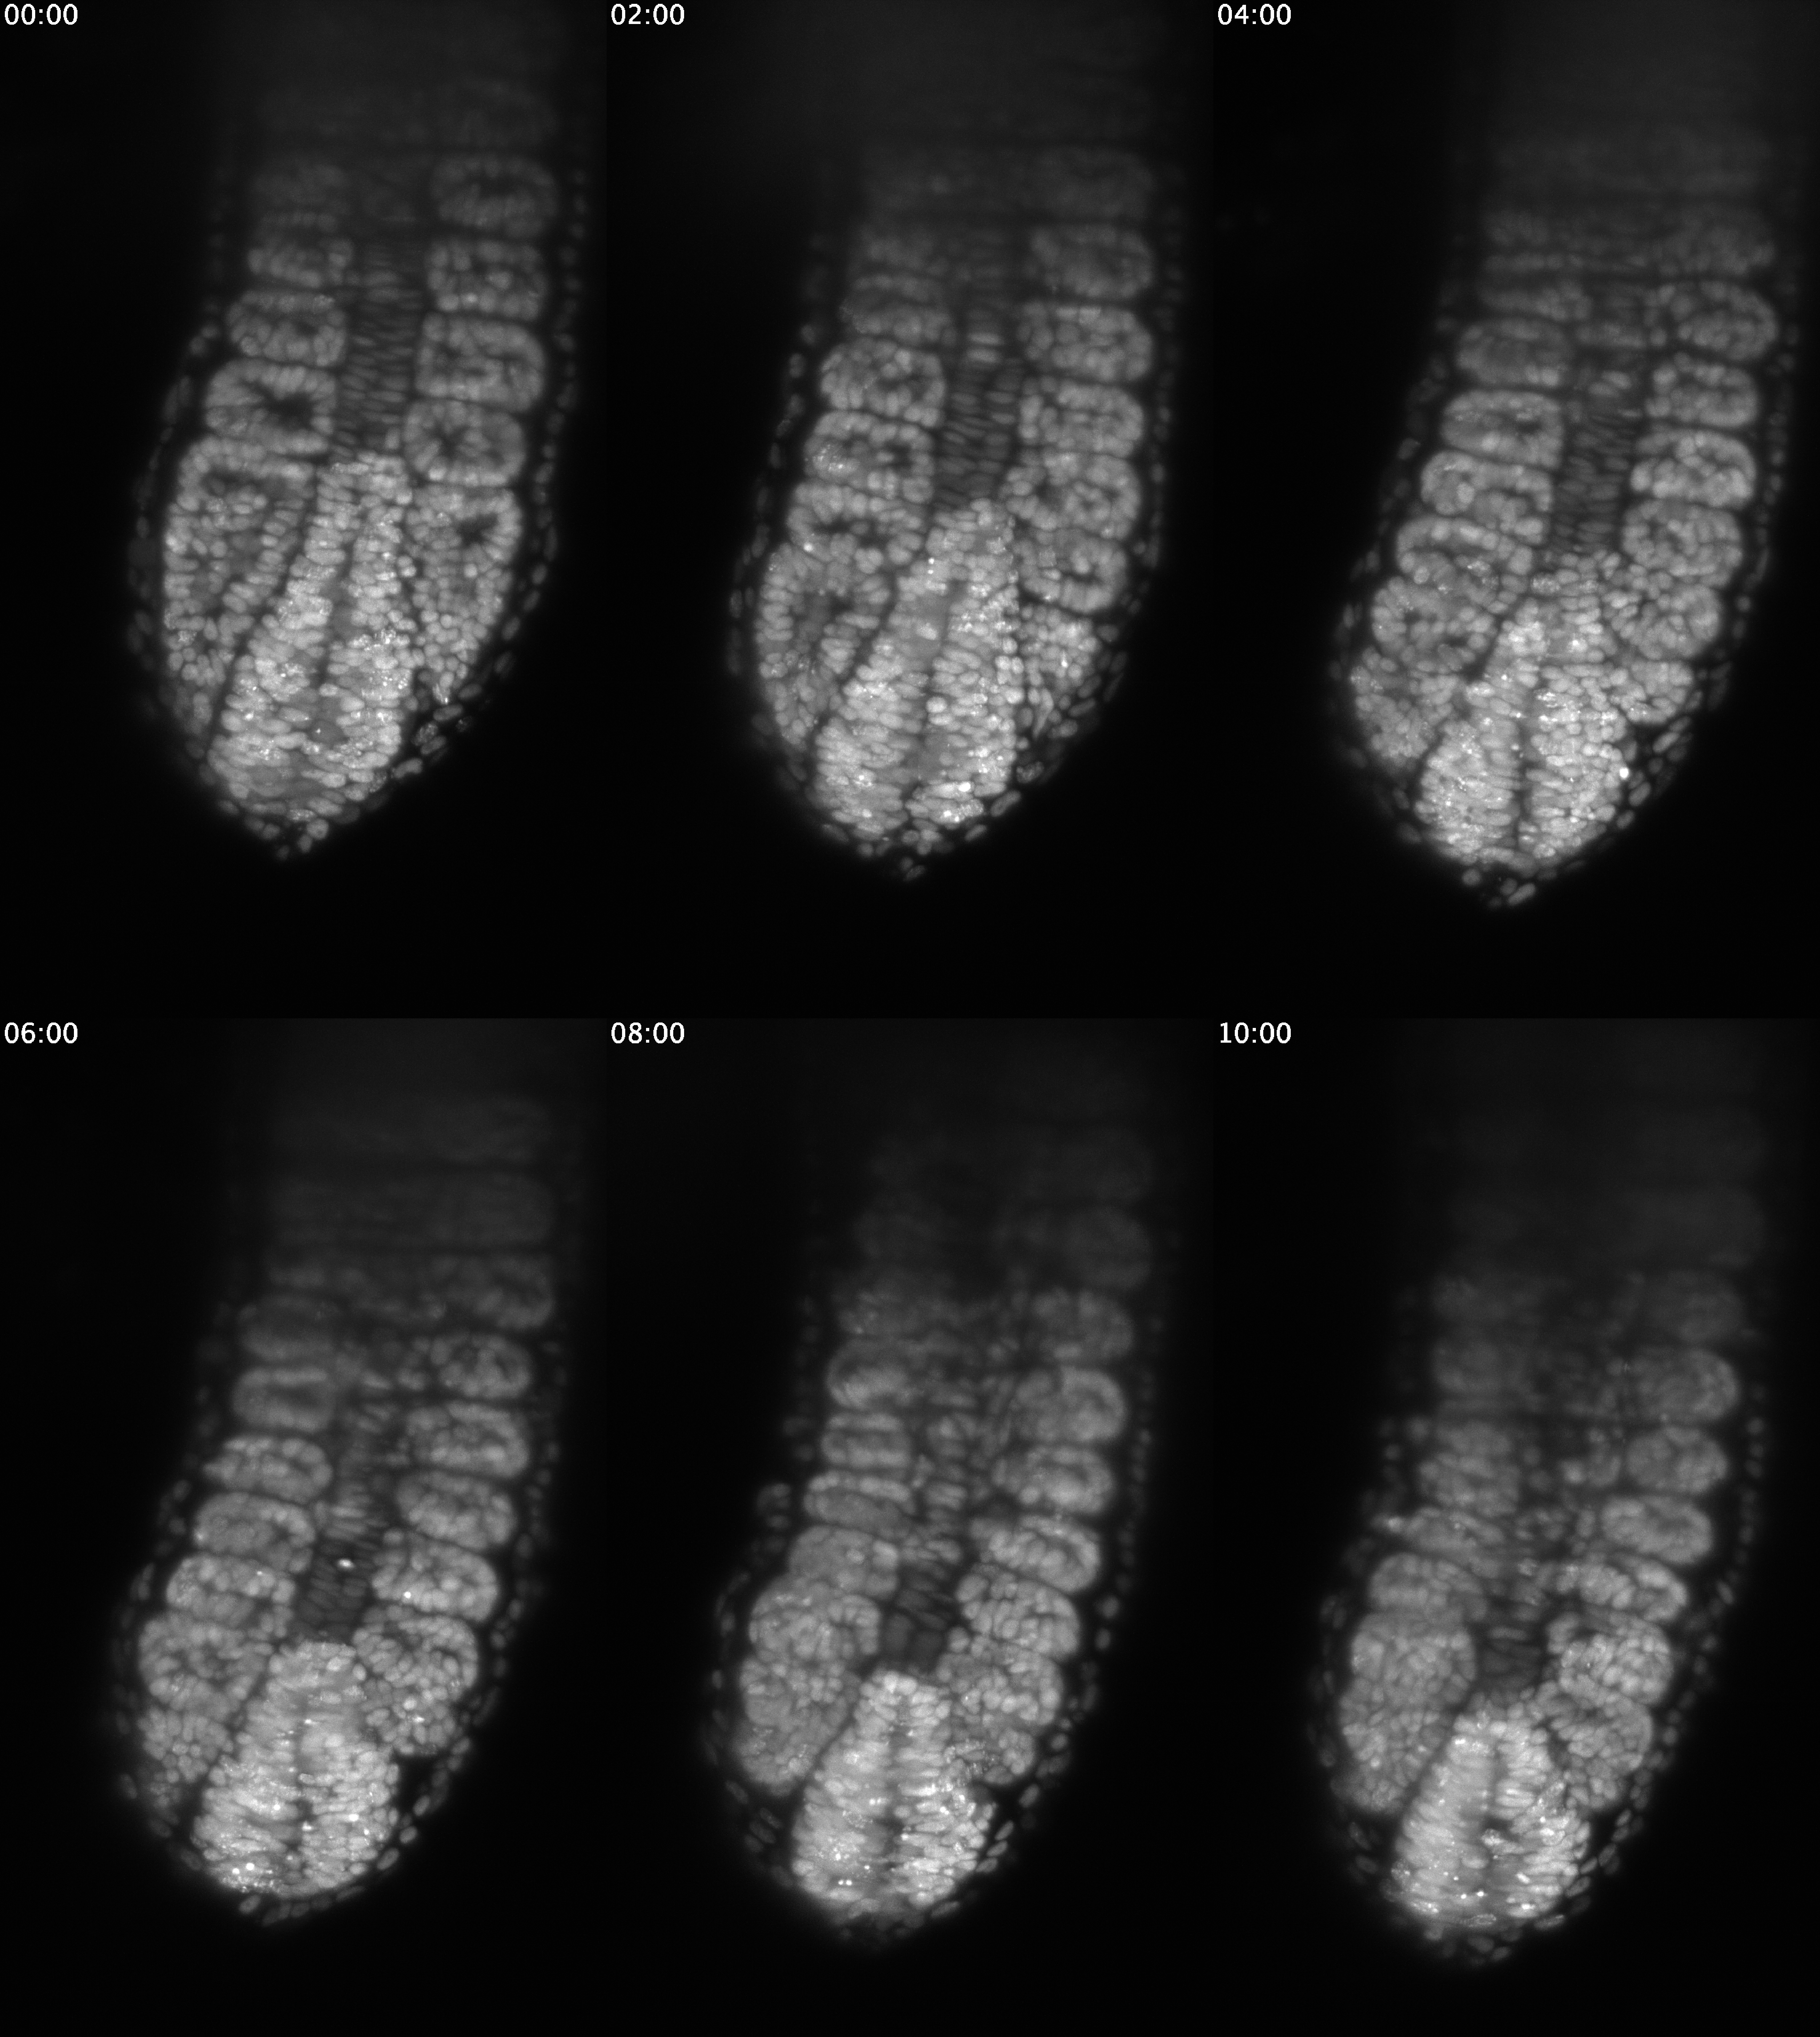
\includegraphics[width=1\linewidth]{figs/somites/ali_fish_seg_compiled} \caption{Time-stamped images of somite segmentation in medaka, generated by Ali Seleit.}\label{fig:somite-seg-ali}
\end{figure}

The period of somite formation is controlled by a molecular oscillator, known as the `segmentation clock', which drives waves of gene expression in the Notch, fibroblast growth factor (FGF), and Wnt pathways, forming a signalling gradient that regresses towards the tail in concert with axis elongation (Gomez et al. 2008). Over the course of elongation, the wave period at the tip of the tail increases (i.e.~each somite takes longer to form), and the PSM progressively shrinks until it is exhausted, eventually terminating somite formation (Gomez et al. 2008).

It is not fully understood how the phase waves of the segmentation clock are intially established (Falk et al. 2022). Matsuda et al. (2020) found that period differences between mouse and human occur at the single-cell level (i.e.~not due to intercellular communication), and could be driven by biochemical reaction speeds -- specifically, mRNA and protein degradation rates, transcription and translation delays, and intron and splicing delays. However, the authors did not provide a genetic explanation for why these biochemical reaction rates are different. Expanding on this work, our collaborators Ali Seleit and Alexander Aulehla at EMBL-Heidelberg are exploring the genetic basis of differences in segmentation clock periods. Carina Vibe of the Aulehla group used a CRISPR-Cas9 knock-in approach to establish a medaka \emph{Cab} strain with an endogenous, fluorescing reporter gene (\emph{Her7}-Venus, \textasciitilde1.5 kb in length at the locus 16:28,706,898-28,708,417) for the oscillation signalling pathway.\footnote{This work is yet to be published, but the approach is similar to that described in Seleit, Aulehla, and Paix (2021).} This method allows them to image somite formation and extract quantitative measures for segmentation clock dynamics.

In medaka, it is known that the southern Japanese \emph{Cab} strain and the northern Japanese \emph{Kaga} strain have divergent somite periodicity, where \emph{Kaga}'s tends to be faster, and \emph{Cab}'s slower (\textbf{Figure \ref{fig:F0-Cab-Kaga-HdrR}}). Our collaborators accordingly set up a one-way F2 cross experiment as described in Chapter \ref{MIKK-F2-cross}, using the reporter-carrying \emph{Cab} strain and the \emph{Kaga} strain as the parental F0 strains, in order to identify genetic loci associated with these differences in clock dynamics.



\begin{wrapfigure}{L}{0.5\textwidth}
\includegraphics[width=1\linewidth]{figs/somites/ali_period_F0_Cab_Kaga} \caption{Comparison of period for three inbred medaka strains (\emph{Cab}, \emph{Kaga} and \emph{HdrR}). Kaga's period is lower, and therefore it takes less time to form each somite than \emph{Cab}. Figure generated by Ali Seleit.}\label{fig:F0-Cab-Kaga-HdrR}
\end{wrapfigure}

They inter-crossed the hybrid F1 generation to create a sample of 622 F2 individuals (having selected for the F2 individuals carrying either one or two copies of the \emph{Her7}-Venus reporter gene), imaged the developing embryos of these F2 samples, and used pyBOAT (Schmal, Mönke, and Granada 2022) to extract the oscillation features during somite development. \textbf{Figure \ref{fig:somite-period-ali}} shows a series of raw images used by pyBOAT to track the elongation of a medaka tail during somitogenesis, with the identified posterior tip of the embryo labelled with a blue circle.



\begin{wrapfigure}{R}{0.5\textwidth}
\includegraphics[width=1\linewidth]{figs/somites/ali_compiled_somite_elong} \caption{Screenshots of vertebral elongation in an F2 individual captured by Ali Seleit during imaging. The blue circle represents the point tracked by pyBOAT over time, generating the quantitative phenotype data on period development used in this study.}\label{fig:somite-period-ali}
\end{wrapfigure}

\cleardoublepage

\hypertarget{somite-phenotype}{%
\section{Phenotypes of interest}\label{somite-phenotype}}

\hypertarget{somite-development-period}{%
\subsection{Somite development period}\label{somite-development-period}}

\textbf{Figure \ref{fig:ali-somite-period-lines}} shows the period data generated by pyBOAT for this study, for 100 illustrative F2 samples over 300 minutes. The same data can be represented by boxplots as shown in \textbf{Figure \ref{fig:ali-somite-period-box}}. I experimented with using the F2 individuals' mean period and period intercept as the phenotype of interest. The two measures are highly correlated (\(Pearson's~r =\) 0.84, \(p\) \textless{} 2.2 x 10\textsuperscript{-16}), so after displaying the distributions for both measures in Figure \ref{fig:somite-phenos}, I proceed to only discuss the analysis of period intercept, as it would appear to potentially be more robust to the changes in slope that can be observed in Figure \ref{fig:ali-somite-period-lines}.



\begin{figure}
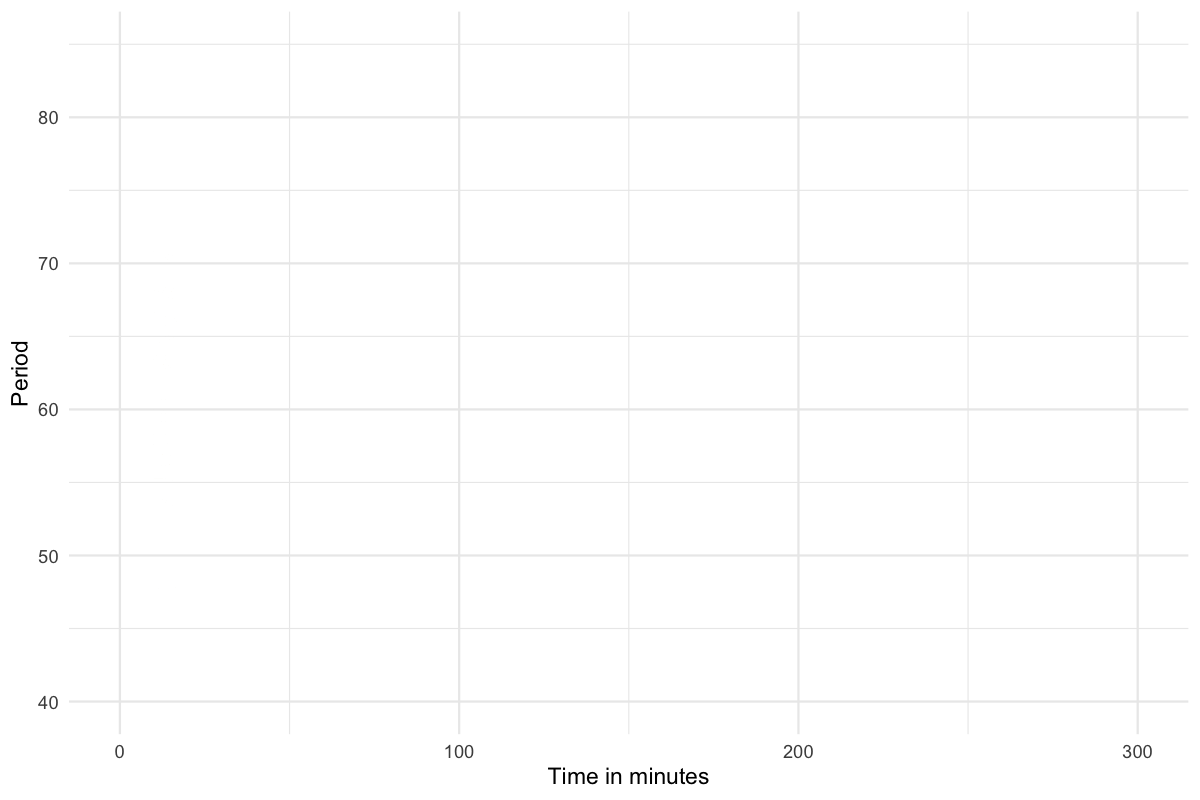
\includegraphics[width=1\linewidth]{figs/somites/ali_period_lines_100fish300mins} \caption{PyBOAT results for 100 illustrative F2 samples, showing the period length in minutes over the course of 300 minutes. Period tends to increase over time, meaning that as the embryo develops, each successive somite takes longer to form. Figure generated by Ali Seleit.}\label{fig:ali-somite-period-lines}
\end{figure}



\begin{figure}
\includegraphics[width=1\linewidth]{figs/somites/ali_F2_mean_period} \caption{Period measurements for 70 F2 individuals displayed as boxplots with each individual's median and interquartile range. Figure generated by Ali Seleit.}\label{fig:ali-somite-period-box}
\end{figure}

\hypertarget{unsegmented-presomitic-mesoderm-area-psm}{%
\subsection{Unsegmented presomitic mesoderm area (PSM)}\label{unsegmented-presomitic-mesoderm-area-psm}}

In the proceeding analyses, I also included a second phenotype of interest: the total area of the presomitic mesoderm prior to the formation of any somite segments (\textbf{PSM area}). As the measure is simply based on the total number of pixels covered by the embryo object, I considered it to be potentially more robust than the period measurements, and therefore included it as a type of positive control for the genetic association analyses on the period phenotype. The measurements for PSM area comparing F0 \emph{Cab} and \emph{Kaga} strains are set out in \textbf{Figure \ref{fig:ali-psm-F0}}.



\begin{wrapfigure}{R}{0.5\textwidth}
\includegraphics[width=1\linewidth]{figs/somites/ali_PSM_Cab_Kaga} \caption{Measurements of unsegmented PSM area in pixels for the F0 individuals from the \emph{Cab} strain (\(N = 19\)) and \emph{Kaga} strain (\(N = 10\)). \emph{Kaga} tends to have a smaller PSM than \emph{Cab}. Figure generated by Ali Seleit.}\label{fig:ali-psm-F0}
\end{wrapfigure}

\hypertarget{comparisons-between-f0-f1-and-f2-generations}{%
\subsection{Comparisons between F0, F1 and F2 generations}\label{comparisons-between-f0-f1-and-f2-generations}}

The distributions across the F0, F1 and F2 generations are unexpected (\textbf{Figure \ref{fig:somite-phenos}}). I rather expected to observe an F2 distribution with a similar median to the F1, and a variance that spanned across the extremes of the F0 strains. Instead, I observed that for the period phenotypes, the F2 generation had a mean that was slightly higher than the median of the higher-period F0 \emph{Cab} strain, and many F2 samples exceed the period values in those F0 samples. Our collaborators assured me that these observations were unlikely to be caused by technical issues. The \emph{Cab} and \emph{Kaga} strains originate from different Japanese medaka populations (southern and northern respectively) that are understood to be at the point of speciation (see Chapter \ref{MIKK-genomes-chap}), so this slower period may be driven by a biological incompatibility between their genomes in cases where they do not have a complete chromosome from each parent (as the F1 generation does). I nevertheless proceeded with the genetic analysis with a view to potentially discovering the reason for this unusual distribution.



\begin{figure}
\includegraphics[width=1\linewidth]{figs/somites/phenotypes} \caption{Comparisons between the F0, F1 and F2 generations for the three phenotypes of interest. Here, the F0 only includes \emph{Cab} individuals. \textbf{A}: period intercept. \textbf{B}: period mean. \textbf{C}: unsegmented PSM area. \(P\)-values are derived from Kruskal-Wallis tests comparing the F2 individuals across microscopes.}\label{fig:somite-phenos}
\end{figure}

Another important issue to note is that the F2 individuals were sequenced using different microscopes, denoted as `AU' and `DB'. Our collaborators noticed that there was a difference between the microscopes in their temperatures of 0.7-0.8°C, translating to a 4-minute difference in the F2 means for the period intercept measure (Kruskal-Wallis = 177.97, \(p\) = 1.34 x 10\textsuperscript{-40}), and a 3.5-minute difference in the F2 means for the period mean measure (Kruskal-Wallis = 141.79, \(p\) = 1.08 x 10\textsuperscript{-32}). This difference would need to be accounted for in the downstream analysis through either adjusting the phenotype prior to running the genetic association model, or by including microscope as a covariate in the model. No significant difference was found for the PSM area.

\hypertarget{inverse-norm-sec}{%
\subsubsection{Inverse-normalisation}\label{inverse-norm-sec}}

To resolve this difference between microscopes for the period intercept data, I elected to transform it for the F2 generation by ``inverse-normalising'' the period intercept within each microscope (\textbf{Figure \ref{fig:invnorm-intercept}}), and used this transformed phenotype for the downstream analysis. Inverse-normalisation is a rank-based normalisation approach which involves replacing the values in the phenotype vector with their rank (where ties are averaged), then converting the ranks into a normal distribution with the quantile function (Wichura 1988). The inverse-normalisation function I used for this analysis is set out in the following \passthrough{\lstinline!R!} code:

\begin{lstlisting}[language=R]
invnorm = function(x) {
  res = rank(x)
  # The arbitrary 0.5 value is added to the denominator below 
  # to avoid `qnorm()` returning 'Inf' for the last-ranked value
  res = qnorm(res/(length(res)+0.5))
  return(res)
}
\end{lstlisting}



\begin{figure}
\includegraphics[width=1\linewidth]{figs/somites/invnorm_intercept} \caption{Comparison of the period intercept phenotype data for the F2 generation before (\textbf{A}) and after (\textbf{B}) inverse-normalisation, with vertical lines marking the mean of each group.}\label{fig:invnorm-intercept}
\end{figure}

\clearpage

\hypertarget{genetic-sequencing-data}{%
\section{Genetic sequencing data}\label{genetic-sequencing-data}}

Our collaborators extracted DNA from the F0, F1, and F2, and sequenced the F0 and F1 samples with the Illumina platform at high coverage (\textasciitilde26x for \emph{Cab} and \textasciitilde29x for \emph{Kaga}), as measured by samtools (Danecek et al. 2021). \textbf{Figure \ref{fig:F0-coverage}} sets out the mean sequencing depth within each chromosome and across the whole genome for the \emph{Cab} and \emph{Kaga} F0 samples. Our collaborators then sequenced the F2 samples at low coverage (\textasciitilde1x), which would be sufficient to map their genotypes back to the genotypes of their parental strains (see section \ref{somite-f2-sequencing} below for further details).



\begin{figure}
\includegraphics[width=1\linewidth]{figs/somites/F0_coverage} \caption{Mean sequencing depth per chromosome for \emph{Cab} and \emph{Kaga} F0 strains, with genome-wide mean depth across all chromosomes shown under the subtitles.}\label{fig:F0-coverage}
\end{figure}

\clearpage

\hypertarget{f0-homozygosity-and-f1-heterozygosity}{%
\section{F0 homozygosity and F1 heterozygosity}\label{f0-homozygosity-and-f1-heterozygosity}}

Before proceeding to map the F2 sequences to the genotypes of the F0 generation, I first investigated the levels of homozygosity in the F0 \emph{Cab} and \emph{Kaga} strains, as this would affect our ability to accurately call the F2 generation. That is to say, for regions where either F0 parent is consistently heterozygous, it would be difficult to determine the parent from which a particular F2 individual derived its chromosomes at that locus. I therefore aligned the high-coverage sequencing data for the F0 \emph{Cab} and \emph{Kaga} strains to the medaka \emph{HdrR} reference (Ensembl release 104, build ASM223467v1) using BWA-MEM2, sorted the aligned .sam files, marked duplicate reads, and merged the paired reads with picard ({``Picard Toolkit''} 2019), and indexed the .bam files with Samtools (Li et al. 2009).

To call variants, I followed the GATK best practices (to the extent they were applicable) (McKenna et al. 2010; DePristo et al. 2011; Van der Auwera and O'Connor 2020) with GATK's HaplotypeCaller and GenotypeGVCFs tools (Poplin et al. 2018), then merged all calls into a single .vcf file with picard ({``Picard Toolkit''} 2019). Finally, I extracted the biallelic calls for \emph{Cab} and \emph{Kaga} with bcftools (Danecek et al. 2021), counted the number of SNPs within non-overlapping, 5-kb bins, and calculated the proportion of SNPs within each bin that were homozgyous.

\textbf{Figure \ref{fig:somite-f0-cab}} is a circos plot generated with circlize (Gu et al. 2014) for the \emph{Cab} F0 strain used in this experiment, featuring the proportion of homozygous SNPs per 5-kb bin (green), and the total number of SNPs in each bin (yellow). As expected for a strain that has been inbred for over 10 generations, the mean homozygosity for this strain is high, with a mean proportion of homozygosity across all bins of 83\%.



\begin{figure}
\includegraphics[width=1\linewidth]{figs/somites/Cab} \caption{Proportion of homozygous SNPs within 5 kb bins in the \emph{Cab} F0 generation genome (green), and number of SNPs in each bin (yellow).}\label{fig:somite-f0-cab}
\end{figure}

\clearpage

However, the levels of homozygosity in the \emph{Kaga} strain used in this experiment was far lower, with a mean homozygosity across all bins of only 31\% (\textbf{Figure \ref{fig:somite-f0-kaga}}). This was a surprise, as it is an established strain of {[}XXXX{]} generations, and we therefore expected the level of homozygosity to be commensurate with that observed in the \emph{Cab} strain. An obvious exception is chr22, for which \emph{Kaga} appears to be homozygous across its entire length.



\begin{figure}
\includegraphics[width=1\linewidth]{figs/somites/Kaga} \caption{Proportion of homozygous SNPs within 5 kb bins in the \emph{Kaga} F0 generation genome (red), and number of SNPs in each bin (yellow).}\label{fig:somite-f0-kaga}
\end{figure}

To determine whether the low levels of observed homozygosity in Kaga was affected by its alignments to the southern Japanese \emph{HdrR} reference, we also aligned the F0 samples to the northern Japanese \emph{HNI} reference (\textbf{Figure \ref{fig:somite-f0-kaga-hni}}. This did not make differences to the levels of observed homozygosity in either sample, which gave us confidence that the low homozygosity observed in \emph{Kaga} was not driven by reference bias. I understand from our collaborators that the low homozygosity of this \emph{Kaga} individual must have resulted from the strain having been contaminated at some stage by breeding with a different inbred strain.



\begin{figure}
\includegraphics[width=1\linewidth]{figs/somites/Kaga_HNI} \caption{Proportion of homozygous SNPs within 5 kb bins in the \emph{Kaga} F0 generation genome when aligned to the \emph{HNI} reference (red), and number of SNPs in each bin (yellow).}\label{fig:somite-f0-kaga-hni}
\end{figure}

\hypertarget{f1-homozygosity}{%
\section{F1 homozygosity}\label{f1-homozygosity}}

I next examined the level of heterozygosity in the F1 generation from the \emph{Cab}-\emph{Kaga} cross. \textbf{Figure \ref{fig:somite-f1}} shows the level of heterozygosity across the genome of the F1 hybrid in brown measured by the proportion of heterozygous SNPs within 5-kb bins (brown), and the number of SNPs in each bin (yellow). Approximately half the chromosomes show inconsistent heterozygosity, with a mean heterozygosity across all bins of 67\%. This lower level of apparent heterozygosity than expected was likely caused by the low levels of homozygosity in the \emph{Kaga} F0 parent.



\begin{figure}
\includegraphics[width=1\linewidth]{figs/somites/F1} \caption{Proportion of heterozygous SNPs within 5 kb bins in the \emph{Cab}-\emph{Kaga} F1 cross (brown), and number of SNPs in each bin (yellow).}\label{fig:somite-f1}
\end{figure}

For the purpose of mapping the F2 sample sequences to the genomes of their parental strains, I selected only biallelic SNPs that were homozygous-divergent in the F0 generation (i.e.~homozygous reference allele in \emph{Cab} and homozygous alternative allele in \emph{Kaga} or vice versa) \emph{and} heterozygous in the F1 generation. The number of SNPs that met these criteria per chromosome are set out in \textbf{Figure \ref{fig:snp-counts-per-chrom}}. The strong homozygosity of \emph{Kaga} on chr22 is likely responsible for the much greater number of loci on that chromosome that can be used for calling genoytpes in the F2 generation, and highlights the importance of the parental strains being highly homozygous when used in experimental crosses such as this.



\begin{figure}
\includegraphics[width=1\linewidth]{figs/somites/snp_counts_per_chr_hdrr} \caption{Number of SNPs per chromosome that were homozygous-divergent in the F0 \emph{Cab} and \emph{Kaga} generations, and heterozygous in the F1 generation.}\label{fig:snp-counts-per-chrom}
\end{figure}

\clearpage

\hypertarget{somite-f2-sequencing}{%
\section{F2 genotyping}\label{somite-f2-sequencing}}

To maximise the efficiency of our sequencing runs, our collaborators ``shallow-sequenced'' the F2 generation with the short-read Illumina platform at a depth of \textasciitilde1x. We then aligned these sequences to the \emph{HdrR} reference with BWA-MEM2 (Vasimuddin et al. 2019), sorted the reads and marked duplicates with Picard ({``Picard Toolkit''} 2019), then indexed the resulting BAM files with samtools (Danecek et al. 2021). Genotyping these shallow sequences with the same method as used for the high-coverage sequences for the F0 and F1 generation would be inappropriate. We therefore used a different method whereby we used \emph{bam-readcount} (Khanna et al. 2022) to count the reads that supported either the \emph{Cab} or the \emph{Kaga} allele for all SNPs that met the criteria described above in section \ref{f1-homozygosity}, summed the read counts within 5 kb blocks, and calculated the frequency of reads within each bin that supported the \emph{Kaga} allele. This generated a value for each bin between 0 and 1, where 0 signified that all reads within that bin supported the \emph{Cab} allele, and 1 signified that all reads within that bin supported the \emph{Kaga} allele. Bins containing no reads were imputed with a value of 0.5.

I then used these values for all F2 individuals as the input to a Hidden Markov Model (HMM) with the software package \emph{hmmlearn} (\emph{Hmmlearn/Hmmlearn} {[}2014{]} 2022), which I applied to classify each bin as one of three states, with state 0 corresponding to homozygous-\emph{Cab}, 1 corresponding to heterozygous, and 2 corresponding to homozygous-\emph{Kaga}. Across each chromosome of every sample, the output of the HMM was expected to produce a sequence of states. Based on previous biological knowledge that crossover events occur on average less than once per chromosome (Haenel et al. 2018) (see \textbf{Figure \ref{fig:zebrafish-co-per-chrom}} for the average crossover rates per chromosome in zebrafish), I expected to observe the same state persisting for long stretches of the chromosome, only changing to another state between 0 and 3 times, and rarely more.



\begin{figure}
\includegraphics[width=1\linewidth]{04-somites_files/figure-latex/zebrafish-co-per-chrom-1} \caption{Crossovers per chromosome based on data provided in Haenel et al. (2018), where ``crossovers per chromosome'' for each chromosome \(c\) was calculated by \(\frac{crossover~rate_{c}(cM / Mb) \times length_{c}(Mb)} {100}\). The medaka genome is shorter in length than zebrafish genome (\textasciitilde800 Mb compared to \textasciitilde1,300 Mb), which according to the authors would suggest that medaka likely has a higher average crossover rate than what is presented in this figure.}\label{fig:zebrafish-co-per-chrom}
\end{figure}

\textbf{Figure \ref{fig:hmm-scat}} shows how adjusting the HMM parameters changed the called genotypes for 10 F2 samples on chromosome 18. Allowing the HMM to train itself for the transition probabilities and emission variances, the HMM produced an apparently noisy output (\textbf{Figure \ref{fig:hmm-scat}A}). Fixing the transition probabilities to make it very likely for a state to transition back to itself rather than to another state.



\begin{figure}
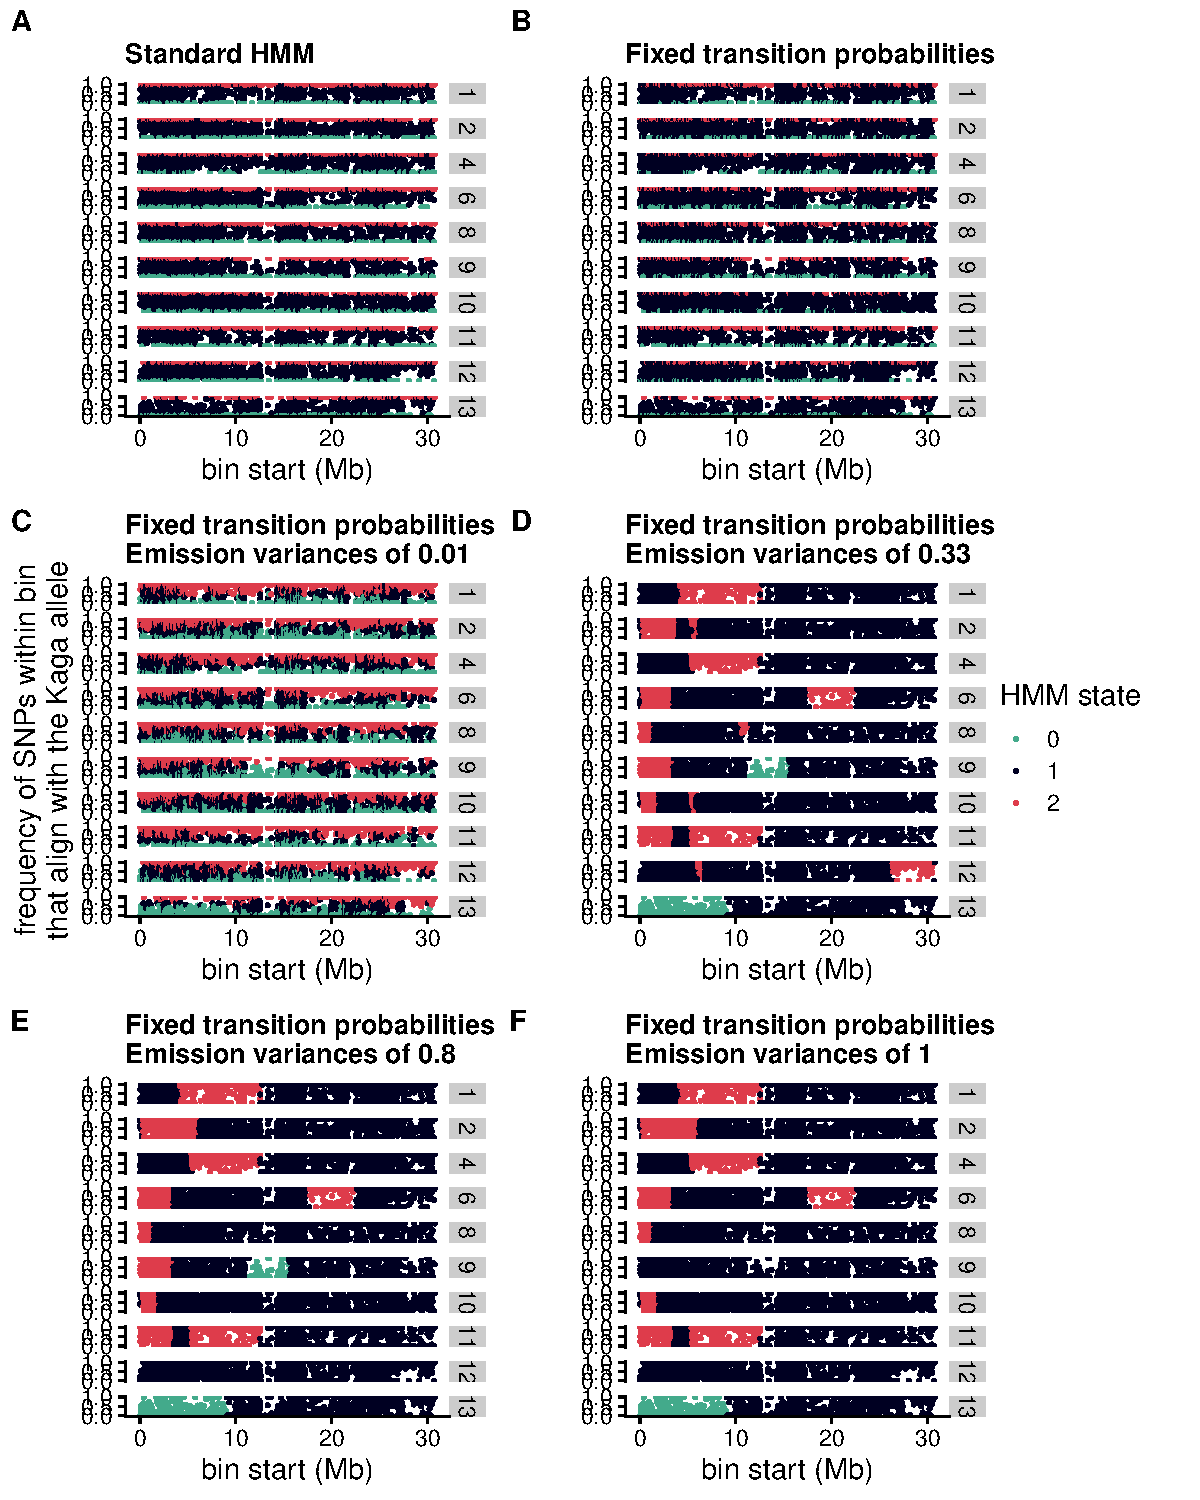
\includegraphics[width=1\linewidth]{figs/somites/scatter_collage} \caption{HMM states called for each bin across chr18 for 10 F2 samples. States 0, 1, and 2 correspond to homozygous \emph{Cab}, heterozygous, and homozygous \emph{Kaga}. Each point represents a 5-kb bin. Y-axis is the proportion of reads within each bin that align to the \emph{Kaga} allele. X-axis is the bp location of the start of each bin. \textbf{A}: Standard HMM with all model parameters trained on the data. \textbf{B}. HMM with fixed transition probabilities of 0→0 or 1→1 or 2→2 = 0.999; 0→1 or 2→1 = 0.00066; 0→2 or 2→0 = 0.000333; 1→0 or 1→2 = 0.0005. \textbf{C}-\textbf{F} retain those transition probabilities but with different fixed emission variances of 0.01 (\textbf{C}), 0.33 (\textbf{D}), 0.8 (\textbf{E}), and 1 (\textbf{F}).}\label{fig:hmm-scat}
\end{figure}

I used these genotype-block calls to generate the recombination karyoplot shown in \textbf{Figure \ref{fig:karyo-wi-missing}}, with homozygous-\emph{Cab} blocks in green, heterozoygous blocks in navy blue, and homozygous \emph{Kaga} blocks in red. Missing calls are blank, where the vertical blank lines indicate that the region could not be called for any F2 individuals, likely due to an insufficient number of informative SNPs residing in those 5-kb blocks; and horizontal blank lines indicate that the sample could not be called, likely due to low sequencing coverage for that sample.



\begin{figure}
\includegraphics[width=1\linewidth]{figs/somites/karyoplot_wi_missing} \caption{Recombination blocks in 622 F2 samples based on the ratio of reads mapping to either the \emph{Cab} or \emph{Kaga} allele within 5-kb bins, with homozygous-\emph{Cab} blocks in green, heterozoygous blocks in navy blue, and homozygous \emph{Kaga} blocks in red. Most blocks show 0-2 crossover events, as expected, with some regions showing higher numbers of crossovers interpreted as noise. Unfilled regions are those with no state called by the HMM due to a lack of reads mapping to SNPs within those 5-kb bins.}\label{fig:karyo-wi-missing}
\end{figure}

In the downstream analysis, I excluded the 22 samples that showed poor coverage across the genome. For the remaining samples, I ``filled'' the bins with missing genotypes based on the call of the previous called bin, or if unavailable (e.g.~the missing bin was at the start of the chromosome), then the next called bin (\textbf{Figure \ref{fig:karyo-no-missing}}; note that this figure retains the low-coverage samples that were excluded from further analysis to allow for a direct comparison with \textbf{Figure \ref{fig:karyo-wi-missing}}). I used these filled genotype calls for the association tests described below in section \textbf{\ref{somite-assoc-tests}}. These karyoplots show interesting recombination patterns for several chromosomes. The reporter gene resides on chr16 \textasciitilde28.7Mb, so given the F2 individuals were selected for the reporter gene, as expected, all but one F2 individual are called as either homozygous-\emph{Cab} or heterozygous at that locus, with that single exception being a genotyping error. Moreover, the selection for homozygous-\emph{Cab} or heterozygous genotypes at that locus has caused a strong skew towards those genotypes across the whole chromosome.

On chr3, most samples are homozygous-\emph{Cab} for the second half of the chromosome, with a consistent breakpoint around \textasciitilde22 Mb. However, the final fifth of samples which show a different recombination pattern. The samples are sorted based on the order that they were phenotyped and sequenced, so this difference could have been caused by their being generated from different F1 individuals with distinct haplotypes {[}CHECK WITH ALI{]}.



\begin{figure}
\includegraphics[width=1\linewidth]{figs/somites/karyoplot_no_missing} \caption{Recombination blocks in 622 F2 samples based on the ratio of reads mapping to either the \emph{Cab} or \emph{Kaga} allele within 5-kb bins, with homozygous-\emph{Cab} blocks in green, heterozoygous blocks in navy blue, and homozygous \emph{Kaga} blocks in red. Most blocks show 0-2 crossover events, as expected, with some regions showing higher numbers of crossovers interpreted as noise. Bins with missing genotypes were ``filled'' based on the call of the previous called bin, or if unavailable (e.g.~the missing bin was at the start of the chromosome), then the next called bin.}\label{fig:karyo-no-missing}
\end{figure}

\textbf{Figure \ref{fig:prop-sites-total}} shows the proportion of 5-kb bins called as either homozygous-\emph{Cab}, heterozygous, or homozygous-\emph{Kaga} within each F2 sample (points). The ordinary expectation for the ratios would be 0.25, 0.5, and 0.25 respectively. However, we observe a skew towards homozygous-\emph{Cab} and away from homozygous \emph{Kaga}. This was likely caused by the hybrid incompatibility between \emph{Cab} and \emph{Kaga}, given the two strains were derived from populations that are thought to be at the point of speciation (see the previous analysis in \textbf{Chapter \ref{MIKK-genomes-chap}}, section \textbf{\ref{introgression-sec}}).



\begin{figure}
\includegraphics[width=1\linewidth]{figs/somites/prop_sites_total} \caption{Proportions of 5-kb blocks called as either homozygous-\emph{Cab}, heterozygous, or homozygous-\emph{Kaga}.}\label{fig:prop-sites-total}
\end{figure}

\clearpage

\hypertarget{somite-assoc-tests}{%
\section{Genome-wide linkage anlaysis}\label{somite-assoc-tests}}

Finally, I used the called recombination blocks as pseudo-SNPs in a genetic linkage analysis. To detect associations between the pseudo-SNPs and the three phenotypes of interest, I used a mixed linear model (\textbf{MLM}) as implemented in GCTA (Yang et al. 2011). That paper describes the model as follows:

\[
\textbf{y} = \textbf{X}\beta + \textbf{Wu} + \epsilon \\
var(\textbf{y}) = \textbf{V} = \textbf{WW}'\sigma^2_{u} + \textbf{I}\sigma_{\epsilon}^2
\]
Where \(\textbf{y}\) is a \(n\) x 1 vector of phenotypes with \(n\) being the sample size, \(\textbf{W}\) is a standardised genotype matrix, \(\textbf{u}\) is a vector of SNP effects, and \(\epsilon\) is a vector of residual effects. I additionally used the leave-one-chromosome-out implementation of GCTA's MLM, with excludes the chromosome on which the candidate SNP is located when calculating the GRM.

As described above in \textbf{section \ref{somite-phenotype}}, the microscope used to image the embryos (either AU or DB {[}WHAT DO THESE ACRONYMS STAND FOR?{]}) differed by several degrees in heat, which likely caused differences in the measurements observed. We accordingly experimented with including microscope as a covariate, either alone or together with the genotype for the reporter locus (either homozygous or heterozygous), or excluding it altogether. In an attempt to avoid complications resulting from its inclusion, Id also tried inverse-normalising the period phenotype within each microscope group, transforming the phenotype to fit a normal distribution across both microscopes.

To set the significance threshold, I permuted the phenotype across samples using 10 different random seeds, together with all covariates when included, and ran a separate linkage model for each permutation. I then set the lowest \(p\)-value from all 10 permutation as the significance threshold for the non-permuted model. I additionally applied a Bonferroni correction to our \(p\)-values by dividing \(\alpha\) (0.05) by the number of pseudo-SNPs in the model, and set this as a secondary threshold.

\hypertarget{period-intercept}{%
\subsection{Period intercept}\label{period-intercept}}

\textbf{Figure \ref{fig:somite-manhattan}} is a Manhattan plot of the genetic linkage results for the period intercept phenotype, inverse-normalised across microscopes. The regions found to be significant based on the permutations' minimum \(p\)-value are set out in \textbf{Table \ref{tab:somite-sig-int-tbl}}.



\begin{figure}
\includegraphics[width=1\linewidth]{figs/somites/manhattan_intercept} \caption{Manhattan plot of the genetic linkage results for the period intercept phenotype, inverse-normalised across microscopes. Pseudo-SNPs with \(p\)-values lower than the permutation significance threshold are highlighted in red.}\label{fig:somite-manhattan}
\end{figure}

\begin{table}
\centering
\begin{tabular}{rrrrr}
  \hline
 & Chromosome & Bin start & Bin end & Length (kb) \\ 
  \hline
\cellcolor{gray!6}{1} & \cellcolor{gray!6}{3.00} & \cellcolor{gray!6}{31880001.00} & \cellcolor{gray!6}{35420000.00} & \cellcolor{gray!6}{3540.00 }\\ 
  2 & 4.00 & 18090001.00 & 18095000.00 & 5.00 \\ 
\cellcolor{gray!6}{  3} & \cellcolor{gray!6}{10.00} & \cellcolor{gray!6}{2995001.00} & \cellcolor{gray!6}{3690000.00} & \cellcolor{gray!6}{695.00 }\\ 
   \hline
\end{tabular}
\caption{Significant 5-kb bin ranges for period intercept below the minimum p-value from 10 permutations.} 
\end{table}

These regions contained a total of 46,872 SNPs imputed from the genotype of the F0 parental strains.
I ran Ensembl's Variant Effect Predictor (McLaren et al. 2016) over these SNPs to identify those that would be most likely to have functional consequences. The full counts of SNPs falling into each category of `consequence' are set out in \textbf{Table \ref{tab:int-consequence-tbl}}. From this process I identified 38 genes that included a missense variant, 1 that included a missense variant and a start lost (ENSORLG00000014616), ane 1 that included a missense variant and a stop lost (ENSORLG00000015149).

\begin{table}

\caption{\label{tab:int-consequence-tbl}Variant Effect Predictor results for SNPs in the bins.}
\centering
\begin{tabular}[t]{lr}
\toprule
Consequence & Count\\
\midrule
\cellcolor{gray!6}{intron variant} & \cellcolor{gray!6}{47211}\\
intergenic variant & 20045\\
\cellcolor{gray!6}{upstream gene variant} & \cellcolor{gray!6}{7304}\\
downstream gene variant & 5229\\
\cellcolor{gray!6}{3 prime UTR variant} & \cellcolor{gray!6}{1082}\\
\addlinespace
synonymous variant & 694\\
\cellcolor{gray!6}{missense variant} & \cellcolor{gray!6}{383}\\
5 prime UTR variant & 201\\
\cellcolor{gray!6}{splice region variant,intron variant} & \cellcolor{gray!6}{126}\\
missense variant,splice region variant & 19\\
\addlinespace
\cellcolor{gray!6}{splice region variant,synonymous variant} & \cellcolor{gray!6}{17}\\
stop gained & 3\\
\cellcolor{gray!6}{splice donor variant} & \cellcolor{gray!6}{1}\\
start lost & 1\\
\cellcolor{gray!6}{stop lost} & \cellcolor{gray!6}{1}\\
\addlinespace
stop lost,splice region variant & 1\\
\bottomrule
\end{tabular}
\end{table}

Our collaborators then combined these results with bulk RNA-seq that they had performed on F0 \emph{Cab} and \emph{Kaga} individuals, to determine which of these genes are expressed in the tail during embryogenesis. This allowed them to reduce to the list to 29 genes, and a gene ontology analysis of this found that the list of genes was enriched for body axis, somitogenesis, and segmentation (\textbf{Table \ref{tab:psm-final-genes}}). For this list of genes, our collaborators are now in the process of knocking in the protein-altering \emph{Cab} allele into \emph{Kaga} embryos, and \emph{vice versa}, to functionally validate these variants.

\begin{landscape}\begin{table}

\caption{\label{tab:psm-final-genes}Target genes for functional validation expressed in the unsegmented PSM and containing protein alterations. Table generated by Ali Seleit.}
\centering
\resizebox{\linewidth}{!}{
\begin{tabular}[t]{rlll}
\toprule
chromosome\_name & ensembl\_gene\_id & description & Role\\
\midrule
\cellcolor{gray!6}{3} & \cellcolor{gray!6}{ENSORLG00000014656} & \cellcolor{gray!6}{mesoderm posterior protein 2-like} & \cellcolor{gray!6}{Somitogenesis}\\
3 & ENSORLG00000014659 & mesp & Somitogenesis\\
\cellcolor{gray!6}{10} & \cellcolor{gray!6}{ENSORLG00000020474} & \cellcolor{gray!6}{protocadherin 10b} & \cellcolor{gray!6}{Somitogenesis}\\
3 & ENSORLG00000014616 & NA & Possible role in Somitogenesis (MAP-kinase)\\
\cellcolor{gray!6}{10} & \cellcolor{gray!6}{ENSORLG00000020551} & \cellcolor{gray!6}{FAT atypical cadherin 4} & \cellcolor{gray!6}{Possible role in Somitogenesis (PCP, Yap1 regulator)}\\
\addlinespace
10 & ENSORLG00000020531 & neurogenin 1 & Possible role in Somitogenesis (BHLH-TF regulation of Wnt)\\
\cellcolor{gray!6}{3} & \cellcolor{gray!6}{ENSORLG00000015149} & \cellcolor{gray!6}{ADAM metallopeptidase with thrombospondin type 1 motif 18} & \cellcolor{gray!6}{Extracellular matrix}\\
3 & ENSORLG00000015418 & matrix metallopeptidase 15 & Extracellular matrix\\
\cellcolor{gray!6}{10} & \cellcolor{gray!6}{ENSORLG00000020488} & \cellcolor{gray!6}{transforming growth factor beta induced} & \cellcolor{gray!6}{Extracellular matrix}\\
3 & ENSORLG00000028055 & NA &  Signal trasduction (Rho)\\
\addlinespace
\cellcolor{gray!6}{10} & \cellcolor{gray!6}{ENSORLG00000020481} & \cellcolor{gray!6}{ArfGAP with RhoGAP domain, ankyrin repeat and PH domain 3} & \cellcolor{gray!6}{ Signal transduction (GTPase activator RhoGap)}\\
10 & ENSORLG00000020525 & TBC1 domain family member 2A-like & Signal transduction Gtpase activator, cadherin recycling\\
\cellcolor{gray!6}{3} & \cellcolor{gray!6}{ENSORLG00000015260} & \cellcolor{gray!6}{synapse associated protein 1} & \cellcolor{gray!6}{TOR acitivity}\\
10 & ENSORLG00000028553 & NA & NA\\
\cellcolor{gray!6}{3} & \cellcolor{gray!6}{ENSORLG00000015460} & \cellcolor{gray!6}{dpy-19 like C-mannosyltransferase 3} & \cellcolor{gray!6}{glycosylation}\\
\addlinespace
10 & ENSORLG00000022010 & beta-1,4-galactosyltransferase 1 & glycosylation\\
\cellcolor{gray!6}{10} & \cellcolor{gray!6}{ENSORLG00000020498} & \cellcolor{gray!6}{protein NipSnap homolog 3A} & \cellcolor{gray!6}{Mitochondria}\\
10 & ENSORLG00000020494 & nitric oxide associated 1 & Mitochondria\\
\cellcolor{gray!6}{10} & \cellcolor{gray!6}{ENSORLG00000020504} & \cellcolor{gray!6}{ATP-binding cassette sub-family A member 1} & \cellcolor{gray!6}{Metabolism (cholestrol efflux)}\\
3 & ENSORLG00000015118 & phosphorylase kinase regulatory subunit beta & Metabolism\\
\addlinespace
\cellcolor{gray!6}{10} & \cellcolor{gray!6}{ENSORLG00000020493} & \cellcolor{gray!6}{RE1 silencing transcription factor} & \cellcolor{gray!6}{RNA pol II (transcritpion regulation}\\
3 & ENSORLG00000015365 & solute carrier family 7 member 6 opposite strand & RNA pol II (nuclear export)\\
\cellcolor{gray!6}{10} & \cellcolor{gray!6}{ENSORLG00000029052} & \cellcolor{gray!6}{exosome component 3} & \cellcolor{gray!6}{rRNA + RNA binding}\\
3 & ENSORLG00000015278 & adhesion G protein-coupled receptor G3 & G-protein coupled receptor\\
\cellcolor{gray!6}{3} & \cellcolor{gray!6}{ENSORLG00000015287} & \cellcolor{gray!6}{adhesion G-protein coupled receptor G5} & \cellcolor{gray!6}{G-protein coupled receptor}\\
\addlinespace
10 & ENSORLG00000025674 & matrin-3 & inner nuclear protein (chromatin architecture\\
\cellcolor{gray!6}{10} & \cellcolor{gray!6}{ENSORLG00000023325} & \cellcolor{gray!6}{matrin-3} & \cellcolor{gray!6}{inner nuclear protein (chromatin architecture}\\
10 & ENSORLG00000022388 & poly(A) binding protein interacting protein 2 & Translation repressor\\
\cellcolor{gray!6}{3} & \cellcolor{gray!6}{ENSORLG00000015096} & \cellcolor{gray!6}{integrin alpha FG-GAP repeat containing 1} & \cellcolor{gray!6}{NA possibly T cell activation}\\
\bottomrule
\end{tabular}}
\end{table}
\end{landscape}

\hypertarget{psm-area}{%
\subsection{PSM area}\label{psm-area}}

\textbf{Figure \ref{fig:psm-manhattan}} is a Manhattan plot of the genetic linkage results for the PSM area phenotype. The regions found to be significant based on the permutations' minimum \(p\)-value are set out in \textbf{Table \ref{tab:somite-sig-psm-tbl}}, although they exceed the Bonferroni correction threshold as well. I note that this \textasciitilde6 Mb significant region on chromosome 3 does not overlap at all with the significant region discovered for the period intercept phenotype.



\begin{figure}
\includegraphics[width=1\linewidth]{figs/somites/manhattan_psm_no-covariates} \caption{Manhattan plot of the genetic linkage results for the PSM area phenotype. Pseudo-SNPs with \(p\)-values lower than the permutation significance threshold are highlighted in yellow.}\label{fig:psm-manhattan}
\end{figure}

\begin{table}

\caption{\label{tab:somite-sig-psm-tbl}Significant 5-kb bin range for PSM area below the minimum p-value from 10 permutations.}
\centering
\begin{tabular}[t]{rrrr}
\toprule
CHROM & Bin start & Bin end & Length (kb)\\
\midrule
\cellcolor{gray!6}{3} & \cellcolor{gray!6}{20375001} & \cellcolor{gray!6}{26285000} & \cellcolor{gray!6}{5910}\\
\bottomrule
\end{tabular}
\end{table}

This region contained a total of 29,096 SNPs imputed from the genotype of the F0 parental strains.
I ran Ensembl's Variant Effect Predictor (McLaren et al. 2016) over these SNPs to identify those that would be most likely to have functional consequences. The full counts of SNPs falling into each category of `consequence' are set out in \textbf{Table \ref{tab:psm-consequence-tbl}}. From this process I identified 114 genes that included a missense variant, and 1 that included a both a missense variant and a start lost (ENSORLG00000010863, a centriole, cilia and spindle-associated protein).

\begin{table}

\caption{\label{tab:psm-consequence-tbl}Variant Effect Predictor results for SNPs in the bins.}
\centering
\begin{tabular}[t]{lr}
\toprule
Consequence & Count\\
\midrule
\cellcolor{gray!6}{intron variant} & \cellcolor{gray!6}{23189}\\
intergenic variant & 9171\\
\cellcolor{gray!6}{downstream gene variant} & \cellcolor{gray!6}{8894}\\
upstream gene variant & 8491\\
\cellcolor{gray!6}{3 prime UTR variant} & \cellcolor{gray!6}{2104}\\
\addlinespace
synonymous variant & 1141\\
\cellcolor{gray!6}{missense variant} & \cellcolor{gray!6}{716}\\
5 prime UTR variant & 433\\
\cellcolor{gray!6}{splice region variant,intron variant} & \cellcolor{gray!6}{184}\\
splice region variant,synonymous variant & 18\\
\addlinespace
\cellcolor{gray!6}{missense variant,splice region variant} & \cellcolor{gray!6}{7}\\
stop gained & 2\\
\cellcolor{gray!6}{splice donor variant} & \cellcolor{gray!6}{1}\\
start lost & 1\\
\bottomrule
\end{tabular}
\end{table}

Our collaborators then combined these results with bulk RNA-seq that they had performed on F0 \emph{Cab} and \emph{Kaga} individuals, to determine which of these genes are expressed in the unsegmented tail during embryogenesis. This allowed them to reduce to the list to 96 genes, although they were not apparently associated with a specific gene ontology. As with the period intercept phenotype, our collaborators are now in the process of knocking in the \emph{Cab} allele into \emph{Kaga} embryos, and \emph{vice versa}, to functionally validate these variants.

\hypertarget{references}{%
\chapter*{References}\label{references}}
\addcontentsline{toc}{chapter}{References}

\hypertarget{refs}{}
\begin{CSLReferences}{1}{0}
\leavevmode\vadjust pre{\hypertarget{ref-danecekTwelveYearsSAMtools2021}{}}%
Danecek, Petr, James K Bonfield, Jennifer Liddle, John Marshall, Valeriu Ohan, Martin O Pollard, Andrew Whitwham, et al. 2021. {``Twelve Years of {SAMtools} and {BCFtools}.''} \emph{GigaScience} 10 (2): giab008. \url{https://doi.org/10.1093/gigascience/giab008}.

\leavevmode\vadjust pre{\hypertarget{ref-depristoFrameworkVariationDiscovery2011}{}}%
DePristo, Mark A., Eric Banks, Ryan Poplin, Kiran V. Garimella, Jared R. Maguire, Christopher Hartl, Anthony A. Philippakis, et al. 2011. {``A Framework for Variation Discovery and Genotyping Using Next-Generation {DNA} Sequencing Data.''} \emph{Nature Genetics} 43 (5, 5): 491--98. \url{https://doi.org/10.1038/ng.806}.

\leavevmode\vadjust pre{\hypertarget{ref-falkImagingOnsetOscillatory2022}{}}%
Falk, Henning J, Takehito Tomita, Gregor Mönke, Katie McDole, and Alexander Aulehla. 2022. {``Imaging the Onset of Oscillatory Signaling Dynamics During Mouse Embryo Gastrulation.''} \emph{Development (Cambridge, England)} 149 (13): dev200083. \url{https://doi.org/10.1242/dev.200083}.

\leavevmode\vadjust pre{\hypertarget{ref-gomezControlSegmentNumber2008}{}}%
Gomez, C'eline, Ertuğrul M. Özbudak, Joshua Wunderlich, Diana Baumann, Julian Lewis, and Olivier Pourqui'e. 2008. {``Control of Segment Number in Vertebrate Embryos.''} \emph{Nature} 454 (7202, 7202): 335--39. \url{https://doi.org/10.1038/nature07020}.

\leavevmode\vadjust pre{\hypertarget{ref-gridleyLongShortIt2006}{}}%
Gridley, Thomas. 2006. {``The Long and Short of It: {Somite} Formation in Mice.''} \emph{Developmental Dynamics} 235 (9): 2330--36. \url{https://doi.org/10.1002/dvdy.20850}.

\leavevmode\vadjust pre{\hypertarget{ref-guCirclizeImplementsEnhances2014}{}}%
Gu, Zuguang, Lei Gu, Roland Eils, Matthias Schlesner, and Benedikt Brors. 2014. {``Circlize Implements and Enhances Circular Visualization in {R}.''} \emph{Bioinformatics} 30 (19): 2811--12. \url{https://doi.org/10.1093/bioinformatics/btu393}.

\leavevmode\vadjust pre{\hypertarget{ref-haenelMetaanalysisChromosomescaleCrossover2018}{}}%
Haenel, Quiterie, Telma G. Laurentino, Marius Roesti, and Daniel Berner. 2018. {``Meta-Analysis of Chromosome-Scale Crossover Rate Variation in Eukaryotes and Its Significance to Evolutionary Genomics.''} \emph{Molecular Ecology} 27 (11): 2477--97. \url{https://doi.org/10.1111/mec.14699}.

\leavevmode\vadjust pre{\hypertarget{ref-HmmlearnHmmlearn2022}{}}%
\emph{Hmmlearn/Hmmlearn}. (2014) 2022. {hmmlearn}. \url{https://github.com/hmmlearn/hmmlearn}.

\leavevmode\vadjust pre{\hypertarget{ref-hubaudSignallingDynamicsVertebrate2014}{}}%
Hubaud, Alexis, and Olivier Pourqui'e. 2014. {``Signalling Dynamics in Vertebrate Segmentation.''} \emph{Nature Reviews Molecular Cell Biology} 15 (11, 11): 709--21. \url{https://doi.org/10.1038/nrm3891}.

\leavevmode\vadjust pre{\hypertarget{ref-khannaBamreadcountRapidGeneration2022}{}}%
Khanna, Ajay, David E. Larson, Sridhar Nonavinkere Srivatsan, Matthew Mosior, Travis E. Abbott, Susanna Kiwala, Timothy J. Ley, et al. 2022. {``Bam-Readcount - Rapid Generation of Basepair-Resolution Sequence Metrics.''} \emph{Journal of Open Source Software} 7 (69): 3722. \url{https://doi.org/10.21105/joss.03722}.

\leavevmode\vadjust pre{\hypertarget{ref-kimPeriodSomiteSegmentation2011}{}}%
Kim, Woong, Takaaki Matsui, Masataka Yamao, Makoto Ishibashi, Kota Tamada, Toru Takumi, Kenji Kohno, et al. 2011. {``The Period of the Somite Segmentation Clock Is Sensitive to {Notch} Activity.''} \emph{Molecular Biology of the Cell} 22 (18): 3541--49. \url{https://doi.org/10.1091/mbc.e11-02-0139}.

\leavevmode\vadjust pre{\hypertarget{ref-liSequenceAlignmentMap2009}{}}%
Li, Heng, Bob Handsaker, Alec Wysoker, Tim Fennell, Jue Ruan, Nils Homer, Gabor Marth, Goncalo Abecasis, Richard Durbin, and 1000 Genome Project Data Processing Subgroup. 2009. {``The {Sequence} Alignment/Map ({SAM}) Format and {SAMtools}.''} \emph{Bioinformatics} 25 (16): 2078--79.

\leavevmode\vadjust pre{\hypertarget{ref-matsudaSpeciesspecificSegmentationClock2020}{}}%
Matsuda, Mitsuhiro, Hanako Hayashi, Jordi Garcia-Ojalvo, Kumiko Yoshioka-Kobayashi, Ryoichiro Kageyama, Yoshihiro Yamanaka, Makoto Ikeya, Junya Toguchida, Cantas Alev, and Miki Ebisuya. 2020. {``Species-Specific Segmentation Clock Periods Are Due to Differential Biochemical Reaction Speeds.''} \emph{Science} 369 (6510): 1450--55.

\leavevmode\vadjust pre{\hypertarget{ref-mckennaGenomeAnalysisToolkit2010}{}}%
McKenna, Aaron, Matthew Hanna, Eric Banks, Andrey Sivachenko, Kristian Cibulskis, Andrew Kernytsky, Kiran Garimella, et al. 2010. {``The {Genome Analysis Toolkit}: {A MapReduce} Framework for Analyzing Next-Generation {DNA} Sequencing Data.''} \emph{Genome Research} 20 (9): 1297--1303. \url{https://doi.org/10.1101/gr.107524.110}.

\leavevmode\vadjust pre{\hypertarget{ref-mclarenEnsemblVariantEffect2016}{}}%
McLaren, William, Laurent Gil, Sarah E. Hunt, Harpreet Singh Riat, Graham R. S. Ritchie, Anja Thormann, Paul Flicek, and Fiona Cunningham. 2016. {``The {Ensembl Variant Effect Predictor}.''} \emph{Genome Biology} 17 (1): 122. \url{https://doi.org/10.1186/s13059-016-0974-4}.

\leavevmode\vadjust pre{\hypertarget{ref-Picard2019toolkit}{}}%
{``Picard Toolkit.''} 2019. \emph{Broad Institute, GitHub Repository}. \url{https://broadinstitute.github.io/picard/}; Broad Institute.

\leavevmode\vadjust pre{\hypertarget{ref-poplinScalingAccurateGenetic2018}{}}%
Poplin, Ryan, Valentin Ruano-Rubio, Mark A. DePristo, Tim J. Fennell, Mauricio O. Carneiro, Geraldine A. Van der Auwera, David E. Kling, et al. 2018. {``Scaling Accurate Genetic Variant Discovery to Tens of Thousands of Samples.''} {bioRxiv}. \url{https://doi.org/10.1101/201178}.

\leavevmode\vadjust pre{\hypertarget{ref-schmalAnalysisComplexCircadian2022}{}}%
Schmal, Christoph, Gregor Mönke, and Adri'an E. Granada. 2022. {``Analysis of {Complex Circadian Time Series Data Using Wavelets}.''} In \emph{Circadian {Regulation}: {Methods} and {Protocols}}, edited by Guiomar Solanas and Patrick -Simon Welz, 35--54. Methods in {Molecular Biology}. {New York, NY}: {Springer US}. \url{https://doi.org/10.1007/978-1-0716-2249-0_3}.

\leavevmode\vadjust pre{\hypertarget{ref-seleitEndogenousProteinTagging2021}{}}%
Seleit, Ali, Alexander Aulehla, and Alexandre Paix. 2021. {``Endogenous Protein Tagging in Medaka Using a Simplified {CRISPR}/{Cas9} Knock-in Approach.''} \emph{eLife} 10 (December): e75050. \url{https://doi.org/10.7554/elife.75050}.

\leavevmode\vadjust pre{\hypertarget{ref-vanderauweraGenomicsCloudUsing2020}{}}%
Van der Auwera, Geraldine A., and Brian D. O'Connor. 2020. \emph{Genomics in the Cloud: Using {Docker}, {GATK}, and {WDL} in {Terra}}. {O'Reilly Media}.

\leavevmode\vadjust pre{\hypertarget{ref-vasimuddinEfficientArchitectureawareAcceleration2019}{}}%
Vasimuddin, Md, Sanchit Misra, Heng Li, and Srinivas Aluru. 2019. {``Efficient Architecture-Aware Acceleration of {BWA-MEM} for Multicore Systems.''} In \emph{2019 {IEEE International Parallel} and {Distributed Processing Symposium} ({IPDPS})}, 314--24. {IEEE}.

\leavevmode\vadjust pre{\hypertarget{ref-wichuraAlgorithm241Percentage1988}{}}%
Wichura, Michael J. 1988. {``Algorithm {AS} 241: {The Percentage Points} of the {Normal Distribution}.''} \emph{Journal of the Royal Statistical Society. Series C (Applied Statistics)} 37 (3): 477--84. \url{https://doi.org/10.2307/2347330}.

\leavevmode\vadjust pre{\hypertarget{ref-yangGCTAToolGenomewide2011}{}}%
Yang, Jian, S. Hong Lee, Michael E. Goddard, and Peter M. Visscher. 2011. {``{GCTA}: {A Tool} for {Genome-wide Complex Trait Analysis}.''} \emph{The American Journal of Human Genetics} 88 (1): 76--82. \url{https://doi.org/10.1016/j.ajhg.2010.11.011}.

\end{CSLReferences}

\end{document}
